\documentclass{article}

% if you need to pass options to natbib, use, e.g.:
%     \PassOptionsToPackage{numbers, compress}{natbib}
% before loading neurips_2018

% ready for submission
% \usepackage{neurips_2018}

% to compile a preprint version, e.g., for submission to arXiv, add add the
% [preprint] option:
%     \usepackage[preprint]{neurips_2018}

% to compile a camera-ready version, add the [final] option, e.g.:
     \usepackage[final]{neurips_2018}

% to avoid loading the natbib package, add option nonatbib:
\usepackage[nonatbib]{neurips_2018}
\usepackage[utf8]{inputenc} % allow utf-8 input
\usepackage[T1]{fontenc}    % use 8-bit T1 fonts
\usepackage{hyperref}       % hyperlinks
\usepackage{url}            % simple URL typesetting
\usepackage{booktabs}       % professional-quality tables
\usepackage{amsfonts}       % blackboard math symbols
\usepackage{nicefrac}       % compact symbols for 1/2, etc.
\usepackage{microtype}      % microtypography
\usepackage{graphicx}
\usepackage{float}
\usepackage{longtable}
\usepackage{array}
\newcolumntype{n}{>{\arraybackslash}m{5.3cm}}
\newcolumntype{d}{>{\arraybackslash}m{8cm}}

\title{A data-driven study of physiotherapy for cystic fibrosis: identifying sub-types of airway clearance and physical activity patterns using unsupervised clustering}

% The \author macro works with any number of authors. There are two commands
% used to separate the names and addresses of multiple authors: \And and \AND.
%
% Using \And between authors leaves it to LaTeX to determine where to break the
% lines. Using \AND forces a line break at that point. So, if LaTeX puts 3 of 4
% authors names on the first line, and the last on the second line, try using
% \AND instead of \And before the third author name.

%\author{%
%  David S.~Hippocampus\thanks{Use footnote for providing further information
%    about author (webpage, alternative address)---\emph{not} for acknowledging
%    funding agencies.} \\
%    I think we need to keep anonymous for our submission\\
%  Department of Computer Science\\
%  Cranberry-Lemon University\\
%  Pittsburgh, PA 15213 \\
%  \texttt{hippo@cs.cranberry-lemon.edu} \\
  % examples of more authors
  % \And
  % Coauthor \\
  % Affiliation \\
  % Address \\
  % \texttt{email} \\
  % \AND
  % Coauthor \\
  % Affiliation \\
  % Address \\
  % \texttt{email} \\
  % \And
  % Coauthor \\
  % Affiliation \\
  % Address \\
  % \texttt{email} \\
  % \And
  % Coauthor \\
  % Affiliation \\
  % Address \\
  % \texttt{email} \\
%}

\begin{document}


\maketitle

\begin{abstract}
  Children and young people with cystic fibrosis (CYPwCF) are prescribed physiotherapy including daily airway clearance techniques (ACT), and being physically active as part of their treatment. Little is known about how CYPwCF follow this advice in their everyday lives. Physiotherapy has evolved over the decades without the clarity of evidence that would accrue from detailed data. Such data are now being collected as part of Project [Anonymous] which is the largest CF physiotherapy trial in the UK to date. The data come firstly from novel pressure sensors attached to existing ACT devices which measure breathing patterns during normal treatments, and secondly from Fitbit activity trackers which monitor physical activity patterns. In close collaboration with clinical experts, we quantified and characterised this unique ACT and activity data by creating custom features from the waveforms. Using unsupervised learning techniques, We identified meaningful sub-types, with k-means clustering achieving the best performance. We found 4 clusters of ACT data which were sensitive enough to track interventions in ACT routines. Within physical activity data we identified 4 clusters related to daily footsteps  and 5 clusters related to heart rate data.
\end{abstract}

\section{Problem overview}

Cystic Fibrosis (CF) is the most common life-limiting inherited disorder in the UK, affecting approximately 1 in 2500 babies born. It is a systemic genetic disorder that mainly affects the respiratory and digestive systems. In the lungs excessive thick sticky mucus can cause cycles of infection, inflammation and lung damage leading to a deterioration in health. Despite improvements in care, CF remains progressive and incurable. In some cases, lung-transplantation can prolong life, but only half of the current CF population are expected to live to over 40 years old \cite{Keogh2018}.  

To promote clearance of mucus from the lungs, daily physiotherapy is prescribed \cite{Daniels2017}. Airway clearance techniques (ACT) may include a series of  exhalations against resistance into hand-held ACT devices, followed by forced expiration techniques ('huffing') and coughing to improve mucociliary clearance and expel mucous; an exercise which is performed repeatedly \cite{Villanuevaj4574}. ACT is burdensome, with some CYPwCF reporting that ACT is the most burdensome part of having the disease \cite{JamesLindAlliance}. Physiotherapists also encourage children to have a physically active lifestyle, which has been shown to reduce the rate of decline in lung function \cite{Williams2014}. Adherence to physiotherapy has traditionally been assessed via questionnaire or self report, both of which are known to be inaccurate. More objective measures of adherence  have not been widely available, and the evolution of CF physiotherapy has not been informed by this important evidence \cite{Modi2006}.  

Bespoke pressure sensors were developed to attach to existing ACT devices in order to facilitate remote monitoring of ACT undertaken routinely at home. In addition, bespoke games were developed which could be driven by pressure changes from breathing through the sensor. This was in order to investigate if gamification might reduce the treatment burden of ACT or modify ACT adherence or patterns \cite{Jackson2019} \cite{[Anonymised]2019} . Physical activity patterns were also measured using Fitbit activity trackers, which generated granular detail on footsteps and heart rate changes during the day. 

 145 CYPwCF participated in the study [NREC:18-LO-1038] to quantify routine ACTs (using bespoke pressure sensors) and physical activity patterns (from wearing a Fitbit activity tracker), and to study the effects of gamification. This is the largest CF physiotherapy trial in the UK [*******UCL****** ref to meta-analysis of CF trials, or previously largest studies, or any previous data-driven studies?], collecting completely novel daily data about how children follow physiotherapy advice in their everyday lives. The broader goals of the study are to link physiotherapy adherence patterns with clinical outcomes, in order to optimise and personalise treatment. In this paper we describe the challenge of i) quantifying ACT pressure sensor data and Fitbit activity data by creating custom features of the waveforms, and ii) discovering sub-types of ACT and physical activity patterns using clustering techniques. These daily sub-types can be tracked over time, as interventions such as gaming are introduced.  
 
\section{Methods}

\subsection{Trial design and analysis approach}

The 18 month trial used an interrupted time series design, so that the effect of introducing and removing interventions such as gamification could be assessed [[*******UCL****** ref to details of trial design,is this sufficient? NREC:18-LO-1038 ]. Interventions included: introducing feedback to participants on their ACTs (number of breaths per treatment) via a computer tablet application, introducing games, and later removing these interventions. The data presented here is from the first 8x months of the trial. Participants were: [*******UCL****** exact numbers] 65x males and 80x females ranging in age from 6-16 years old, from 3 London hospitals, all of whom consented to participate in the study. All data were completely de-identified for analysis. 
 
Our analysis seeks to find patterns in physiotherapy data. Once these patterns are known, they can be linked with clinical outcomes to determine if certain behaviour patterns are preferable. We do not impose pre-conceived labels such as “good” or “bad” on waveforms, thus we leave open the possibility that what is currently prescribed may not be optimal. As such, the data is unlabelled and we use unsupervised learning approach to achieve this. Unsupervised clustering is becoming an established technique for finding sub-types in physical activity data \cite{physical_activity_patterns_2017} and pressure data relating to respiratory disease []. 

A high-scale data analysis and exploration pipeline was built in R in a secure analysis environment.  

\subsection{Collaboration, trust and interpretability}

Many applications of machine learning to medical data fail to explain how (if at all) the expertise of clinicians has been included \cite{Alaa2018}. To address the issues that arise from a lack of collaboration \cite{Vayena2018}, \cite{Challen231}, \cite{Char2018}, \cite{Ahmad2018} our methodology involved close collaboration between data scientists and CF experts, making every data decision jointly. We used a novel approach of involving at least one clinical expert in engineering “stand-ups” every day over the course of building the data analysis pipeline (7 months). We only considered features that were meaningful to clinicians, and we balanced traditional statistical evaluation metrics, with what was interpretable to clinicians.  

\subsection{Feature engineering}

\subsubsection{Breath data description}

ACT treatments commonly involve around 10 sets of 10 exhalation breaths into an ACT device. Participants generally used 1 of 4 different ACT devices compatible with the pressure sensor; the Acapella, Aerobika, PariPEP or AstraPEP. Each device produced breaths with a slightly different overall shape, e.g. with small oscillations. Sometimes participants used different devices over different days. Each set helps to loosen mucus, and between sets, patients normally 'huff' and cough to expel it. The treatments are usually performed one or more times per day depending on how well the person is or how much mucus they normally produce; participants did not have identical prescriptions. For the study, the ACT device was fitted with a bespoke wireless pressure sensor sampling pressure at 10~Hz, recording pressure values in time-stamped millibars.  

\subsubsection{Processing breath data}

Several pre-processing steps were performed on the data which were a function of the custom sensor used: including assembling data packets and removing duplicate values. The sensor also introduced significant non-linear baseline drift. Because of the asymmetrical nature of the exhalation peaks and sparsity of the signal, we used a sparsity-based de-noising approach with an asymmetry factor, called BEADS \cite{Ning2014}, which is designed for use with chromatogram waveforms which have a similar form. An example of pre-processing raw ACT data is shown in figure \ref{fig:ACTpreprocessing}.

\begin{figure}[htb]
  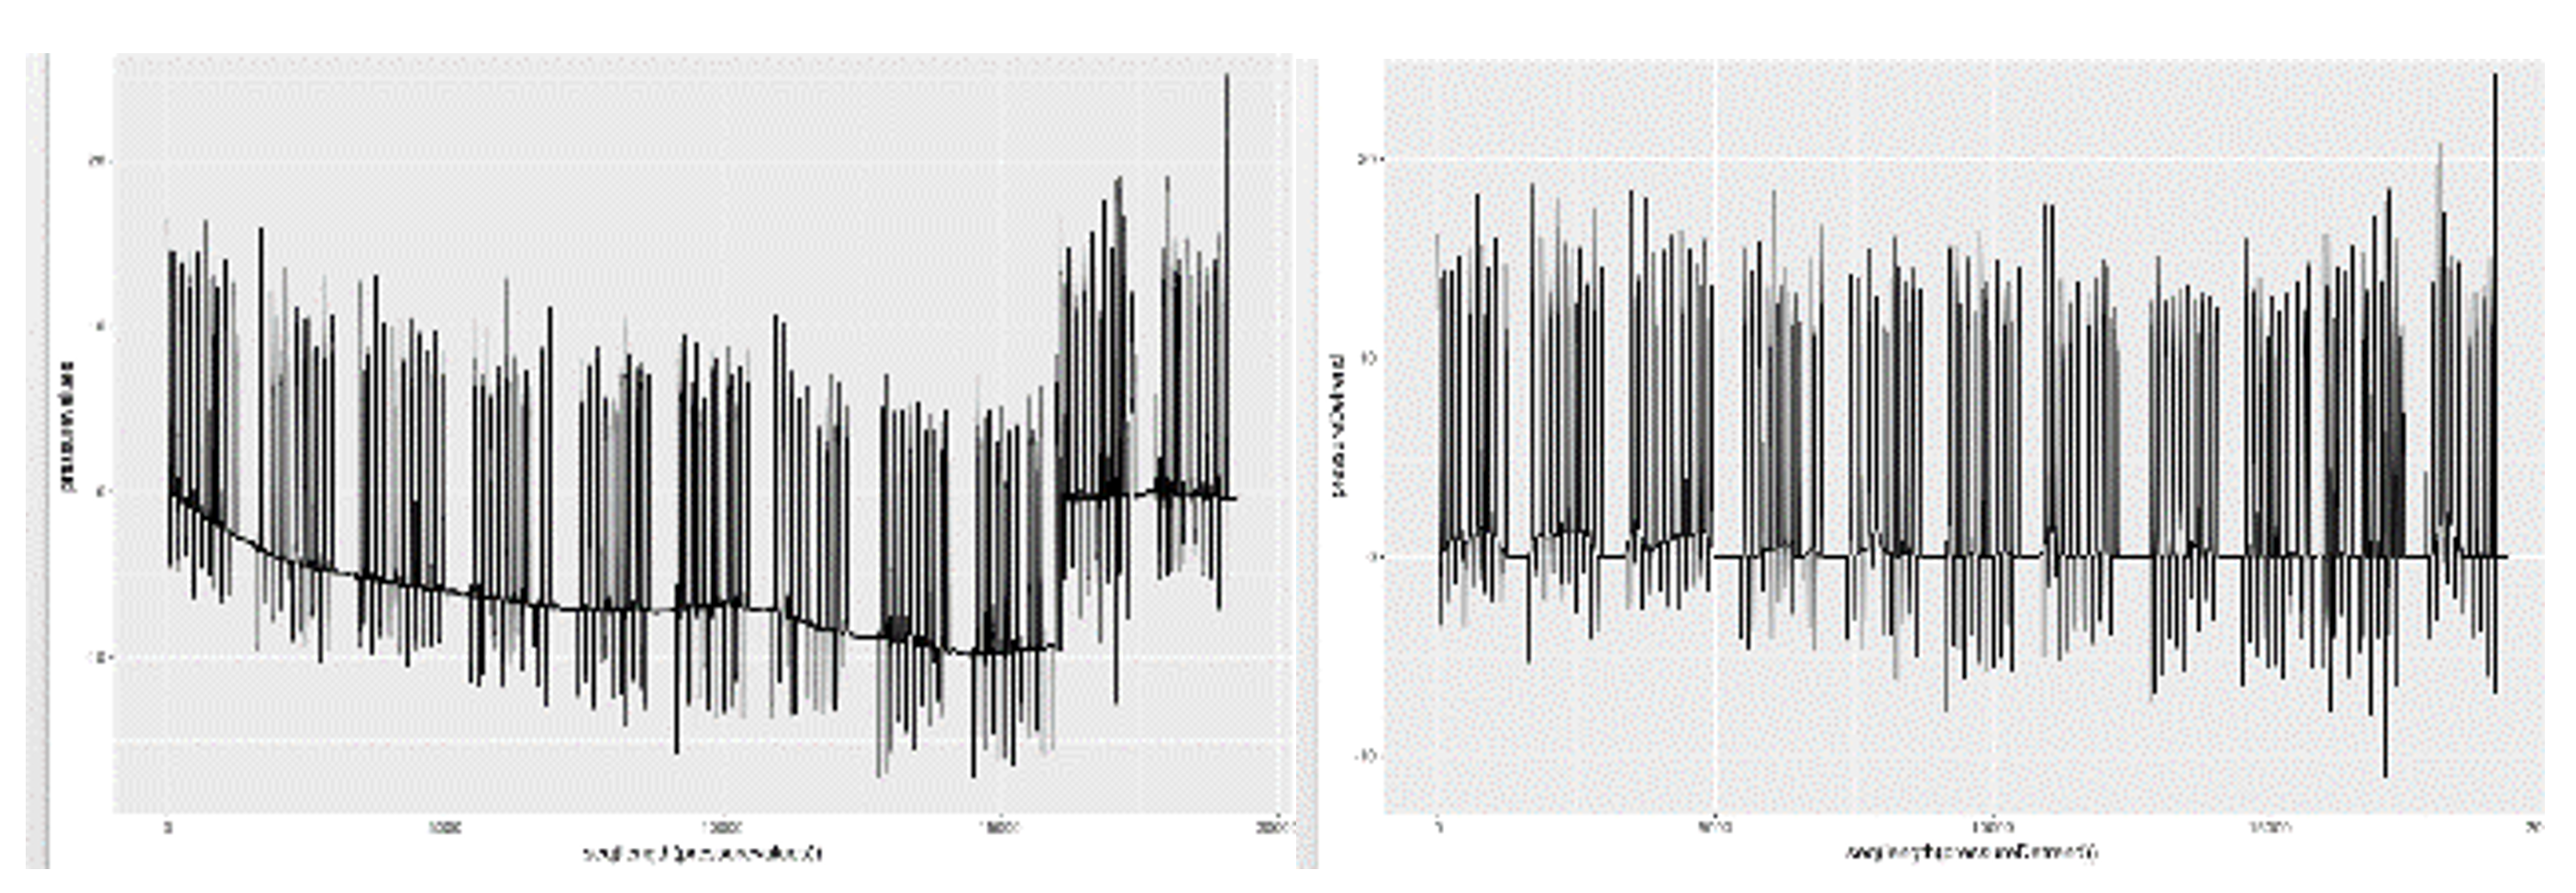
\includegraphics[width=\textwidth]{ACTpreprocessing.png}
  \centering
   \caption{Left: raw ACT data in two packets, with baseline drift. Right: Data packets assembled into a treatment and baseline drift removed. This treatment shows 11 sets of 10 exhalations (the positive peaks), lasting 33 minutes.}
  \label{fig:ACTpreprocessing}
\end{figure}

In total, we recorded 5x,000 sensor readings. This included data from every time the ACT sensor was turned on, including for testing and demonstration. Once we removed readings shorter than 15 seconds, treatments with no breath exhalations, and situations with sensor misuse/malfunction, we were left with 2x,000 ACT treatments for analysis. 

\subsubsection{Featurising breath data}

A typical ACT waveform which has been pre-processed, is shown in figure \ref{fig:individual_breaths}. The defining characteristics of ACT treatments were summarised in a range of features (variables) including: breath count, breath duration, breath amplitude, and treatment duration. In order to derive these features, our breath identification algorithm recognises not only simple breaths, but complex breaths composed of multiple peaks, and having a variety of shapes & oscillations which are characteristic of the 3 different ACT devices used in the study. In addition to mean breath amplitude, we use amplitude standard deviation as a feature, in order to capture inconsistency or disorderliness in physiotherapy. We also identified how many discernible sets were apparent in the treatment. These features are on a per-treatment level. 

\begin{figure}[htb]
  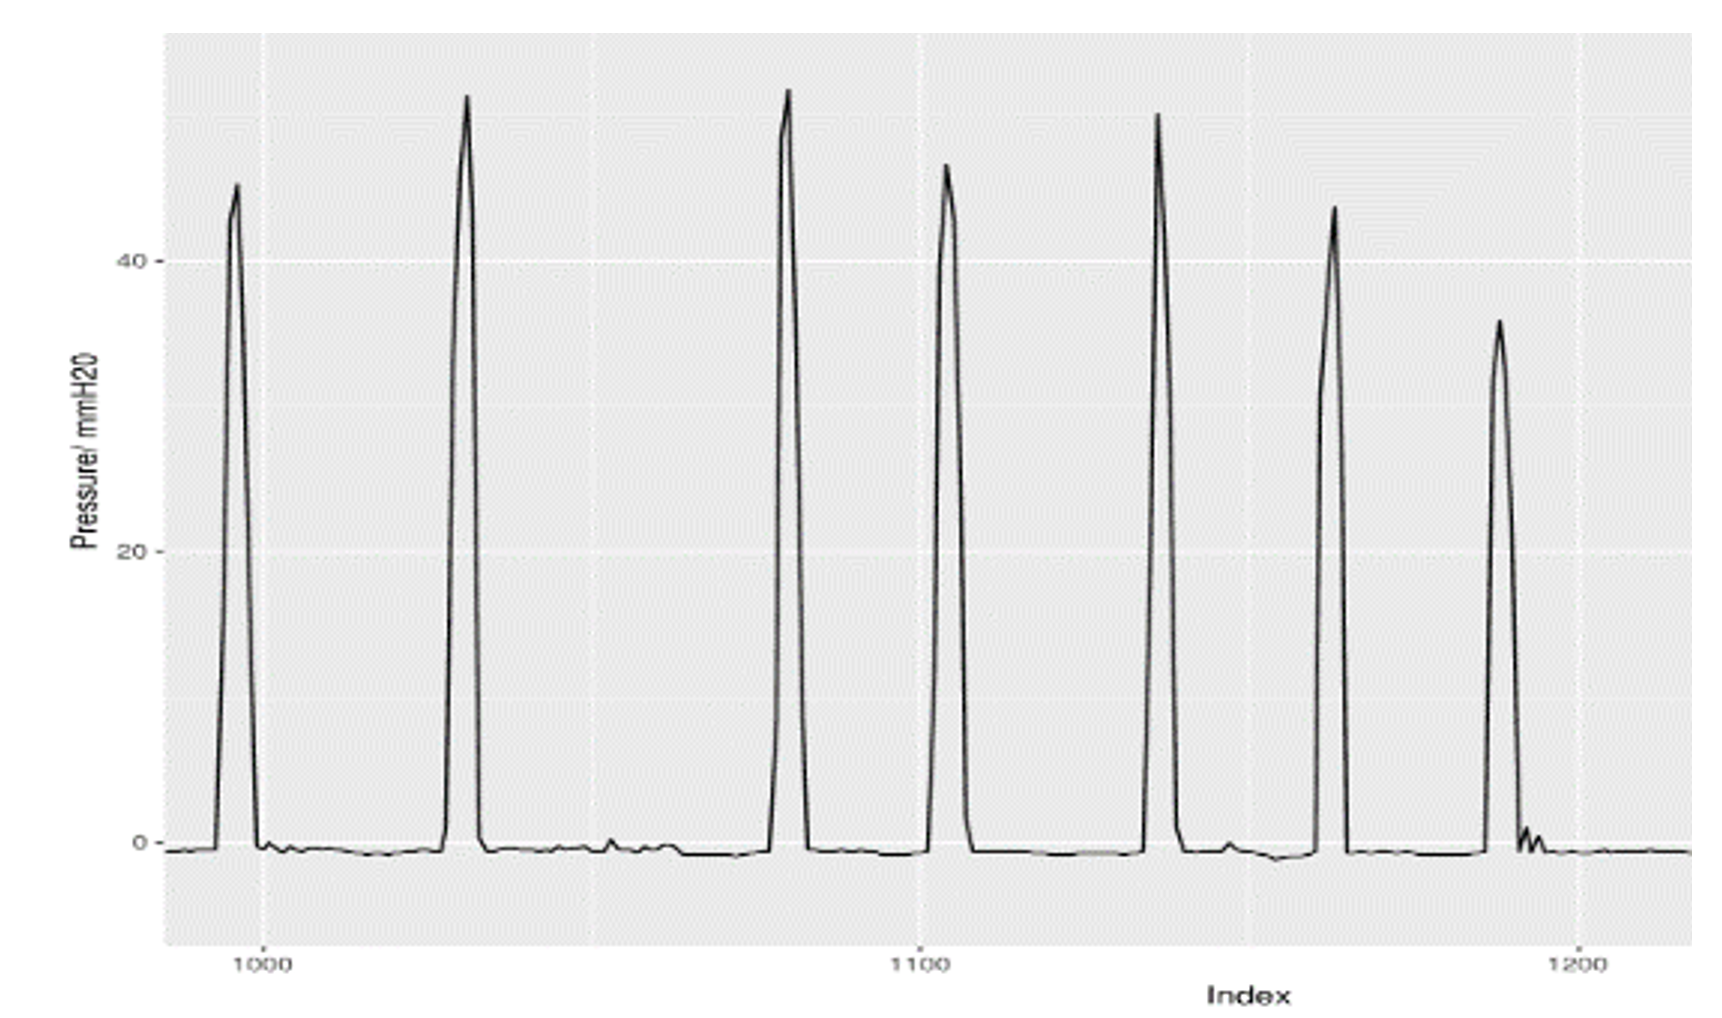
\includegraphics[width=\textwidth]{individual_breaths.png}
  \centering
   \caption{A typical, pre-processed ACT waveform. This treatment is 20 seconds long and contains 7 exhalation breaths.}
  \label{fig:individual_breaths}
\end{figure}

The aforementioned features capture the characteristics of existing treatments. However it is common for prescribed treatments to be skipped, and days with no treatments is an important signal itself. Several features were derived which captured missing data: treatment adherence to date, skipped days since last treatment, rolling adherence over 7 days. These features are on a per-day level, as participants are prescribed 1 or 2 treatments per day. 


\subsubsection{Featurising physical activity data}
The Fitbit activity tracker (Fitbit AltaHR) provided each participant’s step count per minute. While real-time heartbeat data would allow for a detailed analysis of heart rate waveforms, the Fitbit only provides average heart rate, with a variable sampling frequency ranging from 3 to 12 values per minute. To achieve consistent frequency and comparable values, the heart rate values were averaged for each minute. An example of heart rate data is shown in figure \ref{fig:HR}.

\begin{figure}[htb]
  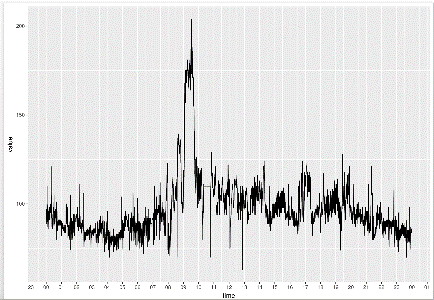
\includegraphics[width=\textwidth]{HR.png}
  \centering
   \caption{One day showing heartrate data with a sustained period of heartrate in MVPA.}
  \label{fig:HR}
\end{figure}

Mindful of these data limitations, we extracted high-level patterns from the minute-averaged waveforms at a day level. The heart rate and steps data sets were featurised using summary statistics per day using counts, frequency and interval values, such as number of minutes in moderate to vigorous intensity physical activities (MVPA) (heart rate above 120 bpm) per day, step cadence (number of steps/minutes of wear) per day, and number of hours with greater than 500 steps per day. 

To account for missing data during times that the Fitbit was not worn, the wear percent of the Fitbit was calculated from the valid heart rate values. This measure was used to select only days with a substantial portion of data for the day (80~\% of wear time from 6~am to 6~pm), resulting in a dataset containing 9760 days used for analysis. The wear time was also used to normalise some features and to obtain step cadence for minutes where heart rate data was present. 

\subsubsection{Clustering to find sub-types}  

All features were verified by clinicians as being meaningful or potentially meaningful. We perform a correlation analysis on all features and removed features which were highly correlated. We use the Hopkins statistic [ref] to measure clustering tendency. Features with a Gaussian distribution were normalised to have mean~=~0 and standard deviation~=~1. In order to visualise the results, we used dimensionality reduction. We used the first two principle components from principal component analysis [ref], Uniform Manifold Approximation and Projection (UMAP) [ref], and t-Distributed Stochastic Neighbor Embedding (T-SNE [ref]. We identified outliers using xxx (Olga) methods and removed less than xxx2~\%, with these cases being recognised as device malfunctions or abnormal behaviour.  

We employed the following clustering methods: k-means, Density-based spatial clustering of applications with noise (DBSCAN) [ref?] and hierarchical clustering.  

\section{Results}

\subsection{Clustering breath waveforms}

\subsubsection{Feature selection for clustering}

Some features were excluded from clustering, but provided interesting physiotherapy insights.  
The number of sets in a treatment were expected to be influential in clustering, as a regular pattern of sets would show close adherence to physiotherapy advice. However we found that less than 20xx\% (Tempest) of treatments had discernible sets, so this feature could not be used. The features used for clustering are shown in table X below, while the full list of features is shown in appendix X. 

\subsubsection{Comparison of clustering techniques}
We compared the three clustering techniques (see appendix) and found the best performance with k-means. 


\begin{figure}[!htb]
  \centering
  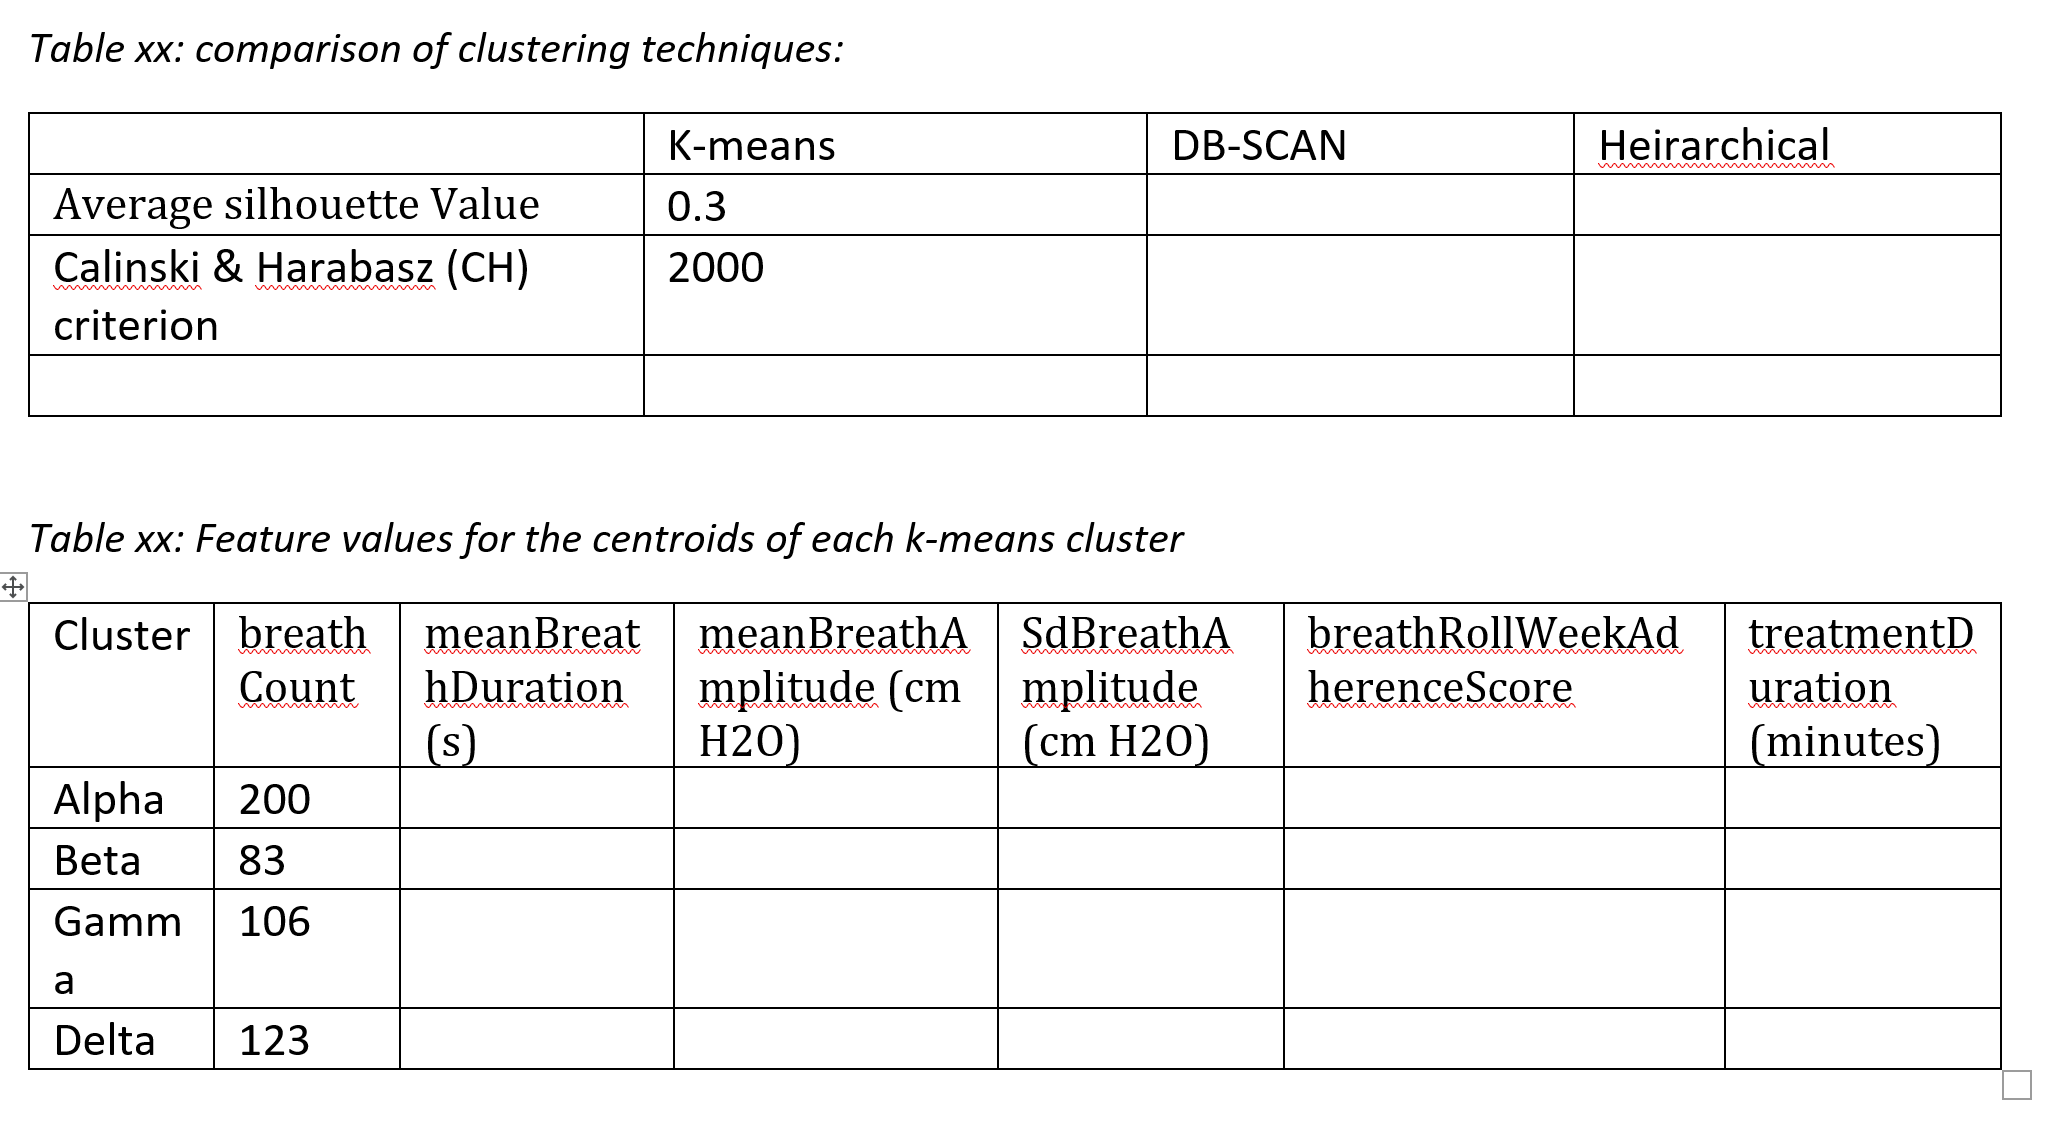
\includegraphics[width=\textwidth]{featureTables.png}
  \caption{To be replaced with a proper table.}
\end{figure}


\subsubsection{ACT K-means clustering results}
The purpose of clustering into sub-types is to summarise how a participant is performing their ACT. We chose k=4 clusters to maximise both silhouette value (average 0.18), and the interpretability of the results. If k is too low, the sub-types are not granular enough, if k is too high it becomes challenging to remember the characteristics of each sub-type. 

The centroid values of the 4 clusters are shown in table X below. Based on these centroids, the four ACT sub-types, which we named alpha, beta, gamma and delta have the following interpretations: 

\begin{itemize}
\item Alpha - Low adherence  ....
\item Beta - High inconsistency ....
\item Gamma -  ....
\item Delta -  ....
\end{itemize}

\subsubsection{ACT clustering validation}

The ACT sub-types should be sensitive enough to capture changes in ACT, particularly during interventions. Figure ~\ref{fig:act_res} shows that clusters are sensitive enough to track changes in a participants' adherence through different study interventions, which validates our approach.

\begin{figure}[!htb]
  \centering
  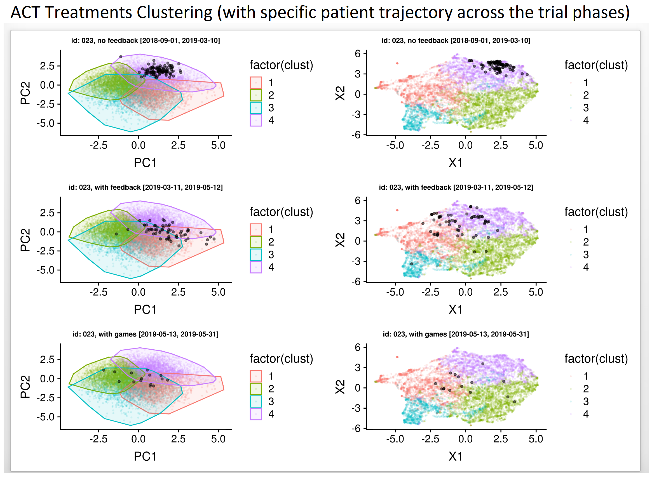
\includegraphics[]{fig_ACT_clust}
  \caption{the four ACT clusters overlaid with a single participant (black), showing that the participant’s cluster membership changes over time. Clustering results are visualised in 2-dimensions using PCA (left) and UMAP (right). The time points are before ACT feedback (number of registered breaths) is introduced (top), after ACT feedback is introduced (middle), and once computer gaming is introduced to ACT routine (bottom). Each point represents one treatment of one participant. }
  \label{fig:act_res}
\end{figure}

We also assessed the clustering stability on different data partitions. Random sampling 80~\% of the data and clustering using k-means provided very similar results with clustering on the full dataset: figure \ref{fig:ACTclusteringon80} shows that the shape of the clusters, cluster centroids as well as Silhouette Coefficients and Calinski-Harabaz Index (2200 v 1770 respectively) were comparable. 

\begin{figure}[!htb]
  \centering
  \caption{K-means clustering results on full dataset (left) and subset of data (right).}
  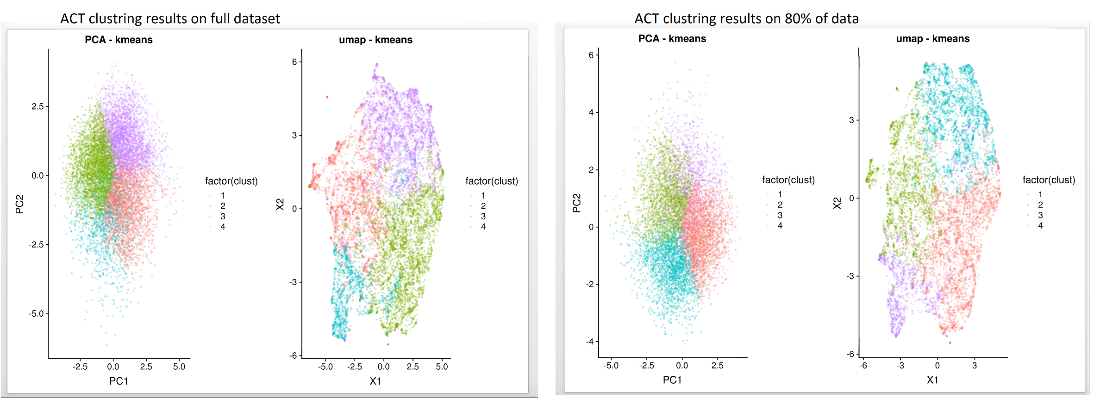
\includegraphics[]{ACTclusteringOn80.png}
  \label{fig:ACTclusteringon80}
\end{figure}

*Not sure about this part. Maybe move to appendix?
We also assessed the validity of the clusters by adding or removing features and checking individual patients’ representation and trajectory in those clusters. Figure \ref{fig:ACTclusteringAB} shows the same patient trajectory for clustering with feature selection A and clustering with feature selection B, which includes two additional features: breath amplitude standard deviation, and rolling weekly adherence score for breath count. It is notable that once computer gaming was introduced to ACT in both cases A and B the same patient moved from cluster with “expected” breath counts per ACT to a cluster characterized by much higher breath counts. This validates that there was a change over time in the patient’s ACT pattern that could be captured. The additional sdBreathAmplitude feature make results more explainable from a clinical point of view, as the original cluster for the patient in Clustering B was characterized by a centroid with the highest sdBreathAmplitude value. 

\begin{figure}[!htb]
  \centering
  \caption{Patient Trajectory on set A of features (without breath amplitude) and set B of features.}
  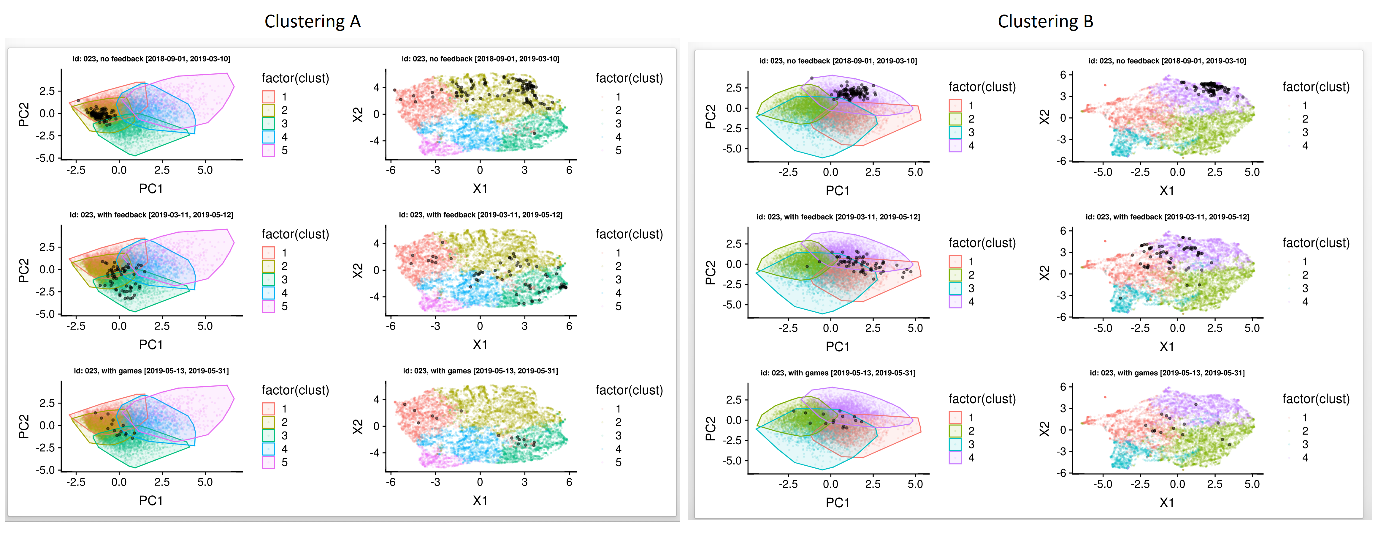
\includegraphics[]{ACTclusteringAB.png}
  \label{fig:ACTclusteringAB}
\end{figure}

\subsection{Clustering physical activity waveforms} 

The purpose of clustering into sub-types is to summarise each participant's physical activity data. Clustering of physical activity data was used to extract daily patterns from the steps and heart rate waveforms and characterise the physical activity levels and patterns of individual patients using a dataset containing 9760 individual days. The different clusters should extract more complex characteristics than the ones which could be obtained by simply combining some of the extracted features.

\subsubsection{Steps clusters}

The following features were used for clustering steps: number of minutes with step count higher than 100 for at least 5 consecutive minutes, the mean of total step count per hour, the step cadence for the periods in MVPA and the number of hours in the day with 0~< ~steps~count~<~500. Features were selected as a result of feature selection, correlation and outlier analysis. Three sub-types were desired for the steps clusters covering small, medium and large amounts of steps activity throughout the day. Four clusters (as shown in figure \ref{fig:stepsClusters}) were chosen in this case to cover these three sub-types as well as a sub-type for the instances with missing data (XS cluster). 

\begin{figure}[htb]
  \centering
  \caption{Steps clusters displayed on the first two principle components.}
  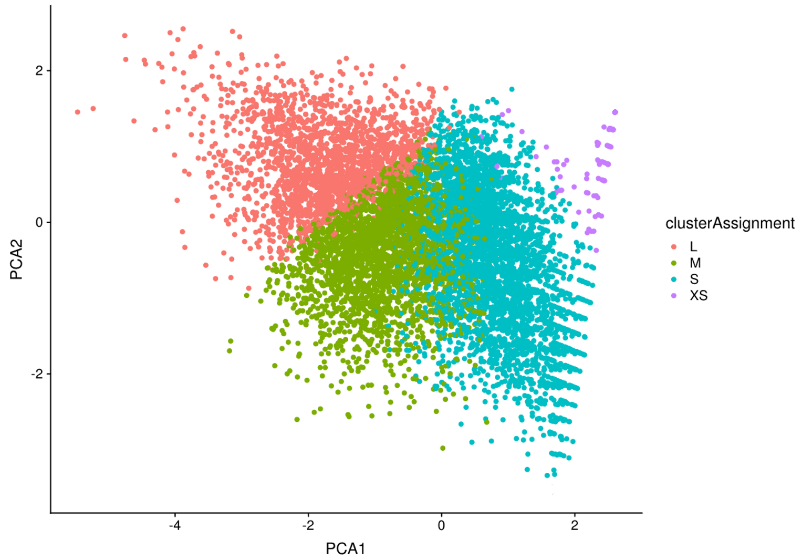
\includegraphics[]{stepsClusters.png}
  \label{fig:stepsClusters}
\end{figure}

\begin{table}[H]
  \caption{Steps Clusters Interpretation}
  \label{steps_inter}
  \centering
  \begin{tabular}{ c|l }
    \toprule
    \cmidrule(r){1-2}
    Cluster name & Cluster Interpretation \\
    \hline
    XS & Waveforms with very little steps activity or high amount of missing data \\
    \hline
    S & Moderate step activity, consistent cadence with few periods of high activity\\
    \hline
    M & Consistent moderate to high step rate with a period of sustained high step activity \\
    \hline
    L & High step rate with longer periods of sustained high step activity \\
    \bottomrule
    \end{tabular}
\end{table}

\subsubsection{Heart rate clusters}

The following were used as features for heart rate clustering: the number of minutes with heart rate higher than 120, coefficient of variation for heart rate values per day, number of time heart rate exceeds 100 and 120, and the median average hourly heart rate. Experiments were carried out with 3, 4 and 5 clusters and the choice of k was based on the cluster interpretability results. The sub-types found when k=5 were the best at identifying more complex patterns and grouping similar waveforms together. 
The five clusters found by K-means (as shown in figure \ref{fig:HRclusters} have the following interpretation: 

\begin{figure}[!htb]
  \centering
  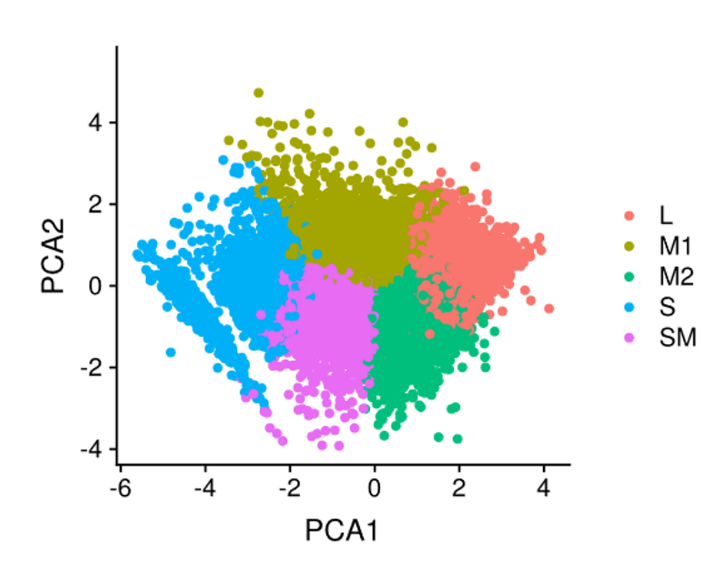
\includegraphics[]{HRclusters.png}
  \caption{PCA of representation of the five heart rate clusters. }
  \label{fig:HRclusters}
\end{figure}


\begin{table}[H]
  \caption{Heartrate Clusters Interpretation}
  \label{hr_inter}
  \centering
  \begin{tabular}{ c|l }
    \toprule
    \cmidrule(r){1-2}
    Cluster name & Cluster Interpretation \\
    \hline
    S & Small heart rate values and heart rate consistently below 120 \\
    \hline
    SM & Consistent variations around 100 with very few spikes in heart rate values \\
    \hline
    M1 &  Waveform with high variability and periods with spikes above 120 \\
    \hline
    M2 & Consistent variations around 100 with spikes in values above 120 \\
    \hline
    L &  Large values around and above 120 \\
    \bottomrule
    \end{tabular}
\end{table}

\subsubsection{Fitbit cluster validation }

The steps and heart rate clusters were validated with clinical experts. The clusters were found to be meaningful and useful ways to categorise the waveforms. Individual waveforms were manually inspected together with the cluster boundaries to ensure consistency across cluster interpretations and the actual cluster characteristics. Additionally, other features that were not included in the clustering analysis were used to validate the clusters and their interpretations. Certain expected conditions were checked against the cluster labels and plotted using the PCA graph such as figure \ref{fig:FitbitClusterValida} below. Cluster boundaries for both steps and heartrate clusters were also utilised to validate the cluster properties and interpretation, these can be found in the Appendix. 

\begin{figure}[!htb]
  \centering
  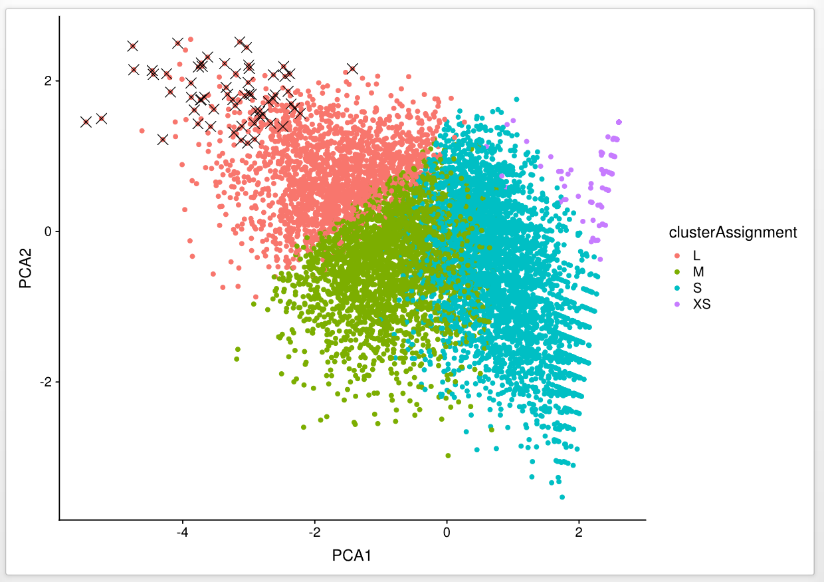
\includegraphics[]{FitbitClusterValidation.png}
  \caption{: Crosses are days with daily cadence above 30 which are all part of the L cluster.}
  \label{fig:FitbitClusterValidation}
\end{figure}


\section{Discussion and conclusion} 

Project [Anonymised] involves collecting novel data about how CF physiotherapy advice on ACTs and physical activity is adhered to in everyday life, information which has never been available to physiotherapists. In close collaboration with CF experts, we developed methods to interrogate and make sense of this data. Project [Anonymised] is an ongoing study, with participation lasting 18 months. 8 months into the trial we do not draw any conclusions, as we do not have an equal number of days of data from patients recruited over 8 months. Instead, we present a framework for analysis, which will empower clinicians to understand how physiotherapy advice is actually adhered to, interpret the impact of interventions such as gamification when the trial is complete., and eventually understand what type of physiotherapy leads to better clinical outcomes. Our framework involves processing the ACT and Fitbit data, deriving clinically meaningful features from it which characterise this novel data, and then using unsupervised clustering to find sub-types of this data. The clusters provide a useful way of tracking participants' trajectories across sub-types over time. 

\section{Usage of tables and figures}
\subsection{Figures}



\subsection{Tables}
\begin{table}
  \caption{Sample table title}
  \label{sample_table}
  \centering
  \begin{tabular}{lll}
    \toprule
    \cmidrule(r){1-2}
    Col1 & Col2 & Col3 \\
    \hline
    a & 0 & z\\
    b & 1 & y \\
    c & 2 & x \\
    \bottomrule
  \end{tabular}
\end{table}

Here is how you can reference a table \ref{sample_table}

\bibliographystyle{abbrv}
% include your .bib file
\bibliography{fizzyo}

\appendix

\section{Appendix : Table of physical activity data features}


\begin{longtable}{  n|d }
\toprule
\cmidrule(r){1-2}
\textbf{Feature Name} & \textbf{Feature description} \\
\hline
\endfirsthead
Minutes wear & Number of minutes in a day with heartrate value present \\
\hline
Percentage of wear & $\frac{\text{Minutes wear}}{24\cdot60}\cdot100\%$\\
\hline
Wear during sleep & Indicator value: 1,  worn during sleep or 0, otherwise \\
\hline
Active hours & Number of hours with a step count > 500  \\
\hline
Low active hours & Number of hours with a step count < 500  \\
\hline
Mean hourly steps & Average of hourly step count \\
\hline
Step count & Total step count per day \\
\hline
Normalised step count & Rate of steps per minute when fitbit is worn \\
 & $\frac{Step Count}{Minutes Worn}$ \\
\hline
 & Number of minutes with step count > 100 with the following constraint: \\
Active Minutes Step 0 & - No minimum of consecutive minutes\\
Active Minutes Step 2 & - At least 2 consecutive minutes > 100 \\
Active Minutes Step 5 & - At least 5 consecutive minutes > 100 \\
Active Minutes Step 10 & - At least 10 consecutive minutes > 100 \\
Active Minutes Step 20 & - At least 20 consecutive minutes > 100 \\
\hline
Active minutes Step for the active period & Number of active minutes with step > 100 from 6am to midnight \\
\hline
Coefficient of Variation Step & Coefficient of variation for steps (removing zero values) at day level \\
 & $CoV = \frac{Standard Deviation}{Mean} * 100$ \\
 \hline
 Normalised step count for periods of : & \\
 - moderate activity & Rate of steps per minute when the heartrate is between 120 and 140. \\ 
 - vigorous activity & Rate of steps per minute when the heartrate is above 140. \\
 - moderate and vigorous activity & Rate of steps per minute when the heartrate is above 120. \\
 - non-moderate and non-vigorous activity & Rate of steps per minute when the heartrate is below 120.\\
 \hline
 Proxy for Resting Heartrate & Mean of the lowest 5 heartrate minutes averages \\
 \hline
 & Number of minutes with heartrate > 120 with the following constraint: \\
Active Minutes Heartrate 0 & - No minimum of consecutive minutes\\
Active Minutes Heartrate 2 & - At least 2 consecutive minutes > 120 \\
Active Minutes Heartrate 5 & - At least 5 consecutive minutes > 120 \\
Active Minutes Heartrate 10 & - At least 10 consecutive minutes > 120 \\
Active Minutes Heartrate 20 & - At least 20 consecutive minutes > 120 \\
\hline
Active minutes Heartrate for the active period & Number of active minutes with heartrate > 100 from 6am to midnight \\
\hline
Coefficient of Variation Heartrate & Coefficient of variation for heartrate (removing zero values) at day level \\
 & $CoV = \frac{Standard Deviation}{Mean} * 100$ \\
 \hline
 Number of threshold switches above 100 & Number of times the heartrate goes above 100 from below this threshold at day level. \\ 
 Number of threshold switches above 120 & Number of times the heartrate goes above 120 from below this threshold at day level. \\ 
 Number of threshold switches above 140 & Number of times the heartrate goes above 140 from below this threshold at day level. \\ 
 \hline
 & Number of minutes with step count > 100 and heartrate > 120 with the following constraint: \\
Active Minutes Step and Heartrate 0 & - No minimum of consecutive minutes\\
Active Minutes Step and Heartrate 2 & - At least 2 consecutive minutes \\
Active Minutes Step and Heartrate 5 & - At least 5 consecutive minutes \\
Active Minutes Step and Heartrate 10 & - At least 10 consecutive minutes \\
Active Minutes Step and Heartrate 20 & - At least 20 consecutive minutes \\
\hline
Heartrate Hourly max, min and median & Maximum. minimum and median of average hourly heartrate. \\
\bottomrule
\end{longtable}

\section{Appendix : Table of ACT treatment features}

\begin{longtable}{ n|d}
\toprule
\cmidrule(r){1-2}
\textbf{Feature Name} & \textbf{Feature description} \\
\hline
Breath Count & Number of breaths the person has made though an ACT  \\ 
 ~ & device during a treatment. A breath is counted if its maximum amplitude is \\ ~ & above the threshold of 8 mm H2O.\\
 \hline
 Mean Breath Amplitude & Average breath amplitude (in mm H2O) during an ACT treatment. \\
 Minimum Breath Amplitude & Similarly minimum, maximum and standard deviation of breath amplitude. \\
 Maximum Breath Amplitude & ~ \\
 Standard Deviation of Breath Amplitude & ~ \\
 \hline
 Mean Breath Duration & Average duration (in seconds) of breath during an ACT treatment. \\ 
 Minimum Breath Duration &  Similarly minimum, maximum and standard deviation of \\ 
 Maximum Break Duration & breath duration in a treatment. \\
 Standard Deviation of Breath Duration & ~ \\
 \hline
 Break Count & Number of breaks (between breaths) in a treatment. \\
 \hline
 Mean Break Duration & Average duration (in seconds) of breaks between breaths. \\ 
 Minimum Break Duration & Similarly minimum, maximum and standard deviation of \\ 
 Maximum Break Duration & breaks duration in a treatment. \\
 Standard Deviation of Break Duration & ~ \\
 \hline
 Set Count & Number of sets in a treatment. Prescribed treatment may have up to 10 \\
 ~ & sets. Set is a group of breaths separated by huffing and coughing activity. \\
 \hline
 Pressure Readings Count & Number of pressure reading registered by ACT device during a treatment. \\
 ~ & Used to filter out "test" device sessions that are not part of a treatment. \\
 \hline
 Pressures Readings Completeness Score & Data completeness score for the day \\
 ~ & If a treatment has less than 150 pressure readings it's completeness \\
 ~ & score is 0. \\
 \hline
 Treatment Duration & Treatment duration (in minutes). \\
 \hline
 Treatment Daily Adherence Score & Number of completed treatments out of the prescribed ones (for the \\
 ~ & given day). \\
 \hline
 Breath Count Daily Adherence Score & Number of registered breaths across all treatments for the given day \\
 ~ & out of the prescribed amount of breaths. \\ 
 \hline
 Treatment Rolling Weekly Adherence Score & Number of completed treatments during the last 7 days (for a given date) \\
 ~ & out of the prescribed number of treatments for this period. \\
 \hline
 Breath Count Rolling Weekly Adherence Score & Number of registered breaths across all treatments during the last 7 days \\
 ~ & (for a given date) out of the prescribed amount of breaths for this period. \\ 
 \hline
 Treatment Weekly Adherence Score & Number of completed treatments during the last calendar week (for a given date) \\
 ~ & out of the prescribed number of treatments for this period. \\
 \hline
 Breath Count Weekly Adherence Score & Number of registered breaths across all treatments during the last calendar week \\
 ~ & (for a given date) out of the prescribed amount of breaths for this period.\\
 \hline
 Cumulative Adherence Score & Cumulative adherence score to date. \\
 ~ & How many in total treatments patient done over a period (since the beginning of the study out the prescribed amount. \\
 \hline
 Breathing Time Percentage & Time in a treatment spent on an exhalation, vs not.\\
 \hline
 Skipped Days Count & Skipped days since the last treatment. \\
 \bottomrule
\end{longtable}

\section{Appendix : Cluster results and metrics for physical activity data}

The tables below show the metrics for the clusters identified for the physical activity data. 

\subsection{Steps clusters}

\subsubsection{K-Means Clustering}

\paragraph{Cluster boundaries}
Cluster boundaries for the four steps clusters can be seen in Figure \ref{fig:stepsBoundaries}.

\begin{figure}[H]
  \centering
  \caption{Steps Cluster Boundaries}
  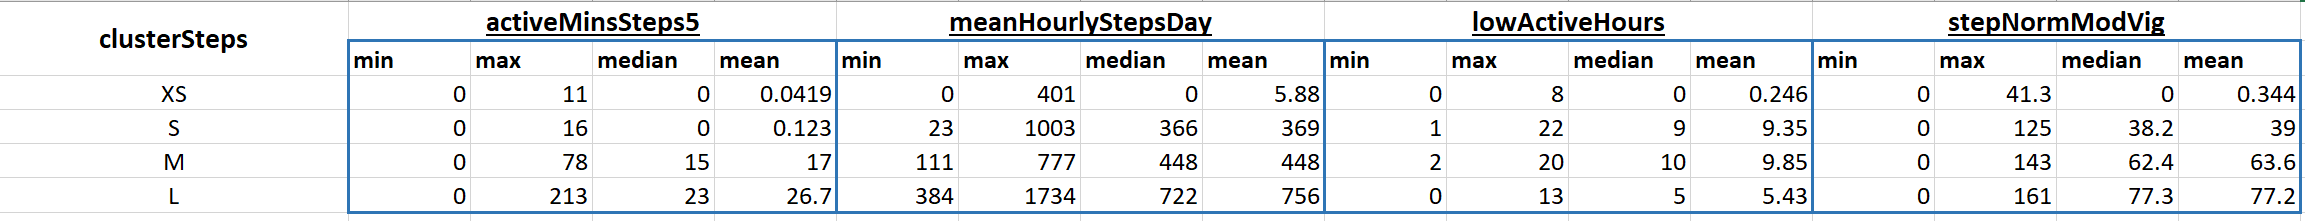
\includegraphics[scale=0.5]{steps_cluster_boundaries.png}
  \label{fig:stepsBoundaries}
\end{figure}

\paragraph{Cluster Metrics}
Calinski-harabasz index for the steps clusters is 6021.14 .

\begin{table}[H]
  \caption{Steps clusters Metrics Kmeans}
  \label{steps_metrics}
  \centering
  \begin{tabular}{ c|c|c}
    \toprule
    \cmidrule(r){1-2}
    Cluster name & Cluster Size & Average Silhouette width \\
    \hline
    XS & 1099 & 0.95 \\
    S & 3942 & 0.34 \\
    M & 2737 & 0.27 \\
    L & 1982 & 0.24 \\
    \bottomrule
    \end{tabular}
\end{table}

\subsubsection{Hierarchical Clustering with complete linkage}

The clustering results using Hierarchical clustering with complete linkage on steps data can be seen in Figure \ref{fig:stepsClustersHC}.

\begin{figure}[htb]
  \centering
  \caption{Steps clusters displayed on the first two principle components obtained using Hierarchical clustering}
  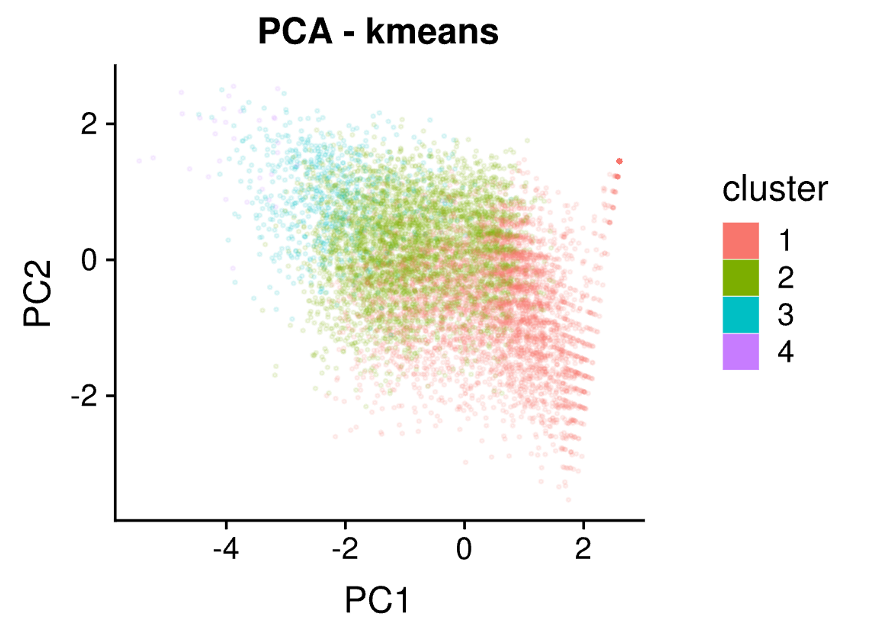
\includegraphics[]{steps_HC_results.png}
  \label{fig:stepsClustersHC}
\end{figure}

Calinski-harabasz index for the steps clusters is 1518.1865 .

\begin{table}[H]
  \caption{Steps clusters Metrics HC}
  \label{steps_metrics}
  \centering
  \begin{tabular}{ c|c|c}
    \toprule
    \cmidrule(r){1-2}
    Cluster number & Cluster Size & Average Silhouette width \\
    \hline
    1 & 4996 & 0.12 \\
    2 & 4056 & 0.11 \\
    3 & 677 & 0.18 \\
    4 & 31 & 0.41 \\
    \bottomrule
    \end{tabular}
\end{table}

\subsection{Heartrate clusters}

\subsubsection{K-Means Clustering}
\paragraph{Cluster boundaries}
Cluster boundaries for the five heartrate clusters can be seen in Figure \ref{fig:hrBoundaries}.

\begin{figure}[H]
  \centering
  \caption{Heartrate Cluster Boundaries}
  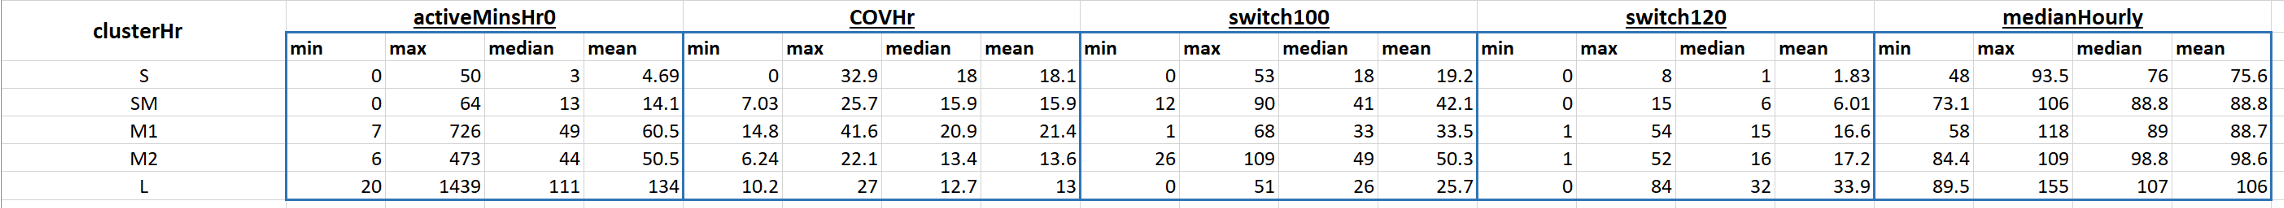
\includegraphics[scale=0.5]{hr_cluster_boundaries.png}
  \label{fig:hrBoundaries}
\end{figure}

\paragraph{Cluster Metrics}
Calinski-harabasz index for the heartrate clusters is 5090.37 .

\begin{table}[H]
  \caption{Heartrate clusters Metrics Kmeans}
  \label{hr_metrics}
  \centering
  \begin{tabular}{ |c|c|c|}
    \toprule
    \cmidrule(r){1-2}
    Cluster name & Cluster Size & Average Silhouette width \\
    \hline
    S & 1246 & 0.28 \\
    SM & 1640 & 0.2 \\
    M1 & 2308 & 0.21 \\
    M2 & 2584 & 0.26 \\
    L & 1982 & 0.33 \\
    \bottomrule
    \end{tabular}
\end{table}

\subsubsection{Hierarchical Clustering with complete linkage}

The clustering results using Hierarchical clustering with complete linkage for the heartrate data can be seen in Figure \ref{fig:hrClustersHC}.

\begin{figure}[htb]
  \centering
  \caption{Heartrate clusters displayed on the first two principle components obtained using Hierarchical clustering}
  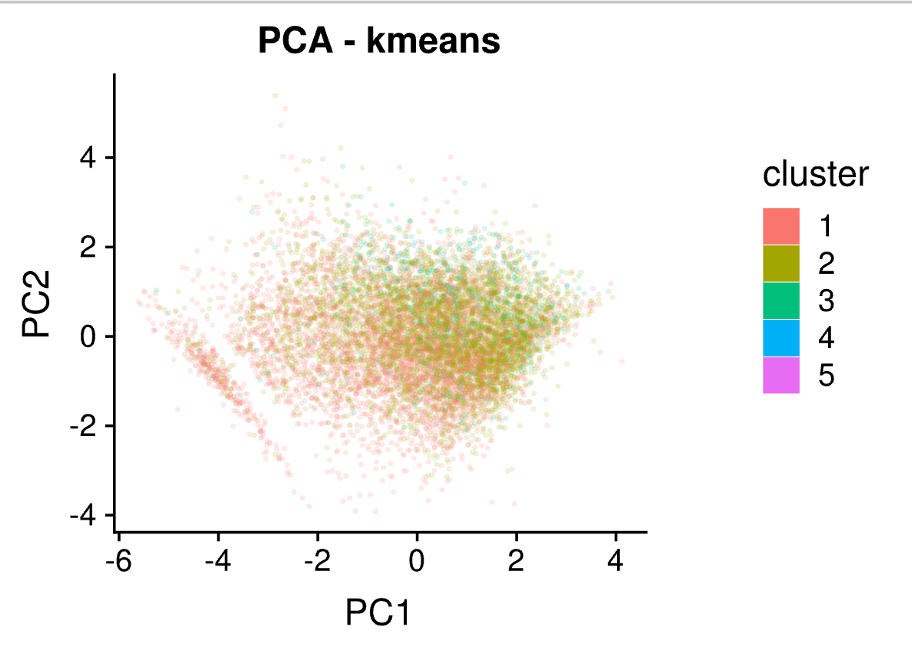
\includegraphics[]{hr_HC_results.png}
  \label{fig:hrClustersHC}
\end{figure}

Calinski-harabasz index for the heartrate clusters is 135.51 .

\begin{table}[H]
  \caption{Heartrate clusters Metrics HC}
  \label{hr_metrics}
  \centering
  \begin{tabular}{ |c|c|c|}
    \toprule
    \cmidrule(r){1-2}
    Cluster number & Cluster Size & Average Silhouette width \\
    \hline
    1 & 4221 & -0.07 \\
    2 & 4901 & -0.06 \\
    3 & 607 & -0.10 \\
    4 & 24 & 0.07 \\
    5 & 7 & -0.06 \\
    \bottomrule
    \end{tabular}
\end{table}

\end{document}